\documentclass{article}
\usepackage{graphicx} % Required for inserting images
\usepackage{listings}
\usepackage{xcolor}
\usepackage{hyperref}

\lstset{
  basicstyle=\ttfamily\small,
  numbers=left,
  numberstyle=\tiny\color{gray},
  keywordstyle=\color{blue},
  commentstyle=\color{green!50!black},
  stringstyle=\color{orange},
  breaklines=true,
  frame=single,
  columns=fullflexible,
  captionpos=b,
}

\title{Operation Final Front++}
\author{Aditya Sai}
\date{Experimental Report and Documentation}

\begin{document}

\maketitle

\section{Introduction}

The objective of the task was to:
\begin{itemize}
    \item Take a graph with nodes and edges (directed) as input
    \item Output the shortest fuel required to reach node $n-1$ from node $0$.
\end{itemize}

The process was broken into two main parts:
\begin{itemize}
    \item Extracting the graph itself, with nodes and edges, into a form where it can be processed further
    \item Applying the algorithm to find the minimum fuel required in the obtained graph.
\end{itemize}

\section{PART A: Extraction}
The initial thought process was to check if OpenCV can directly be used to extract the nodes and edges. The nodes were to be detected using Hough transform and the edges by Canny Edge detection after some preprocessing (such as greyscaling). The node numbers were to be recognised by Tesseract OCR. This would have avoided a lot of hassle which is mostly ML-related.

\begin{lstlisting}[language=Python, caption=calling tesseract OCR]
import pytesseract
pytesseract.pytesseract.tesseract_cmd = r"C:\Program Files\Tesseract-OCR\tesseract.exe"
\end{lstlisting}

\begin{lstlisting}[language=Python, caption=Preprocessing]
image = cv2.imread(image_path)
gray = cv2.cvtColor(image, cv2.COLOR_BGR2GRAY)
blurred = cv2.medianBlur(gray, 5)
\end{lstlisting}

\begin{lstlisting}[language=Python, caption=Detecting circles]
circles = cv2.HoughCircles(
    blurred,
    cv2.HOUGH_GRADIENT,
    dp=1.2,
    minDist=20,
    param1=50,
    param2=30,
    minRadius=10,
    maxRadius=40
)
\end{lstlisting}

\begin{lstlisting}[language=Python, caption=Detecting edges]
edges = cv2.Canny(blurred, 50, 150, apertureSize=3)
lines = cv2.HoughLinesP(
    edges,
    rho=1,
    theta=np.pi / 180,
    threshold=80,
    minLineLength=80,
    maxLineGap=10
)
\end{lstlisting}

\begin{lstlisting}[language=Python, caption=Extracting the nodes with the numbering]
node_ids = {}
for (x, y, r) in circles:
    margin = int(r * 0.8)
    x1, y1 = max(x - margin, 0), max(y - margin, 0)
    x2, y2 = min(x + margin, image.shape[1]), min(y + margin, image.shape[0])
    roi = gray[y1:y2, x1:x2]
    roi = cv2.threshold(roi, 0, 255, cv2.THRESH_BINARY + cv2.THRESH_OTSU)[1]
    text = pytesseract.image_to_string(roi, config='--psm 10 -c tessedit_char_whitelist=0123456789')
    text = text.strip()
    if text.isdigit():
        node_ids[(x, y)] = int(text)
\end{lstlisting}

It was observed that numbers were not being detected with full accuracy using simple Otsu thresholding, so an extra step was added (resizing) and the thresholding was also switched to adaptive thresholding, and it was now mostly error-free.

\begin{lstlisting}[language=Python, caption=Extra steps added in preprocessing]
roi = cv2.resize(roi, None, fx=2, fy=2, interpolation=cv2.INTER_CUBIC)
roi = cv2.adaptiveThreshold(roi, 255, cv2.ADAPTIVE_THRESH_GAUSSIAN_C, cv2.THRESH_BINARY_INV, 11, 2)
\end{lstlisting}

\begin{figure}[h!]
    \centering
    \includegraphics[width=0.5\textwidth]{annotated.png}
    \caption{Canny edge detection seemingly detected whole lines but actually broke them into small chunks.}
    \label{fig:example}
\end{figure}

\begin{figure}[h!]
    \centering
    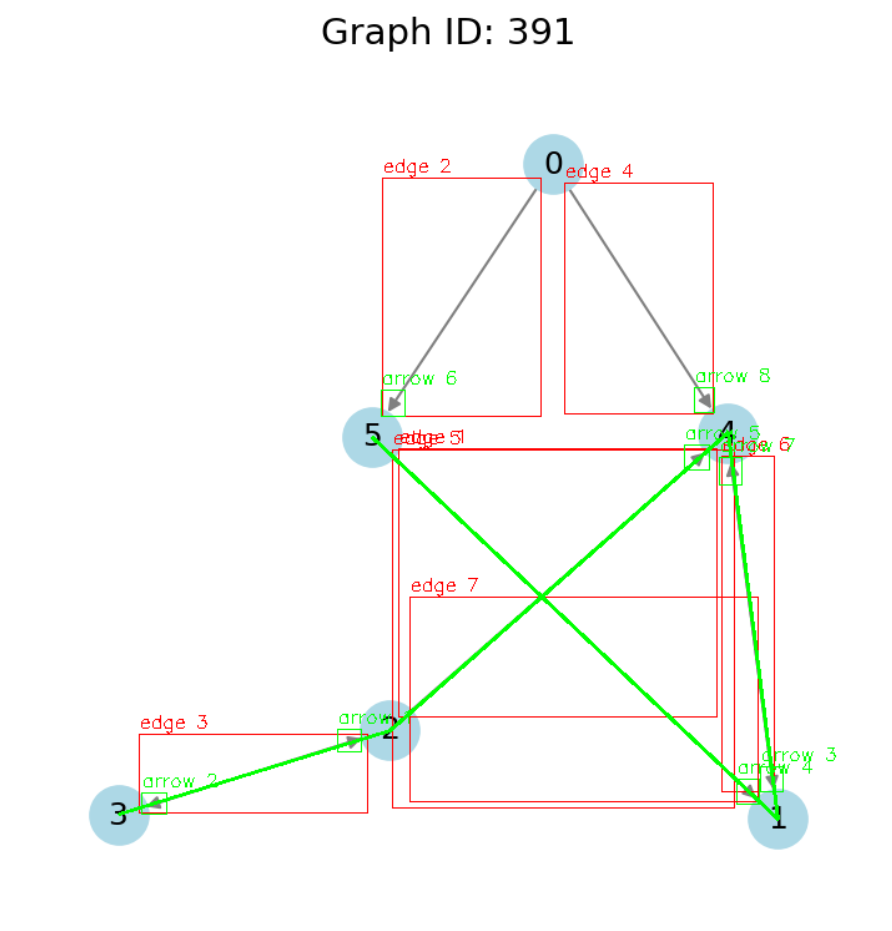
\includegraphics[width=0.5\textwidth]{391_before_preprocessing.png}
    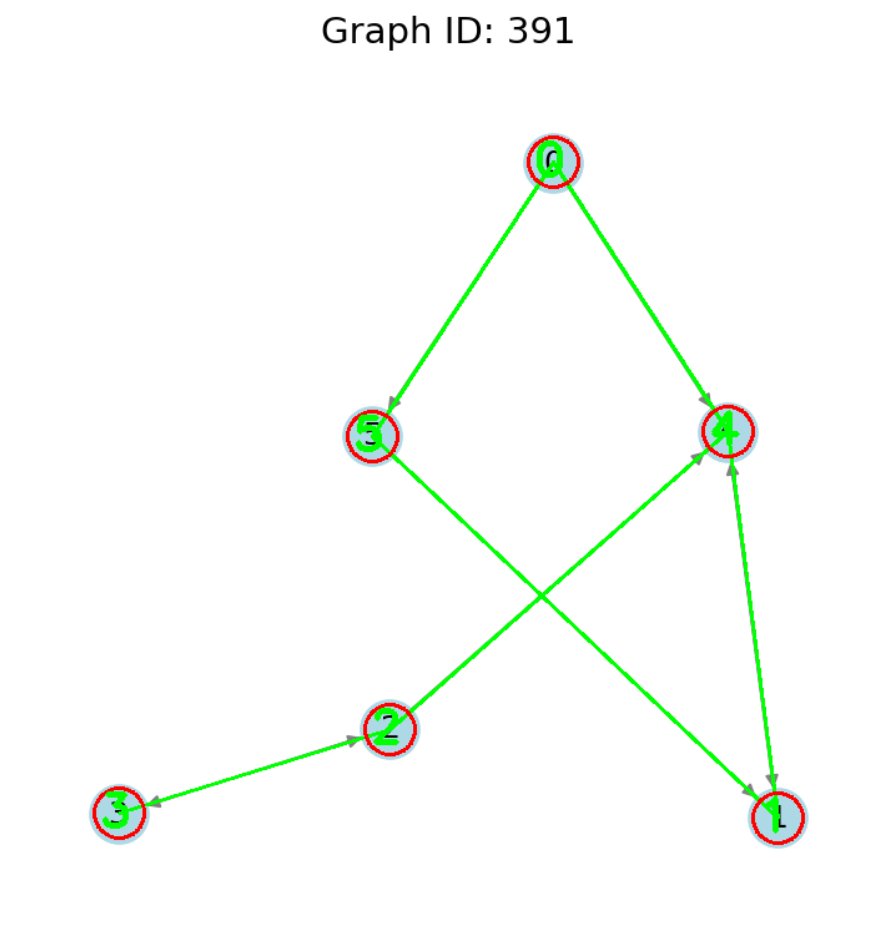
\includegraphics[width=0.5\textwidth]{391_after_preprocessing.png}
    \caption{Analysis: Node 0 was being left out before the preprocessing step was added. The second image shows the result from the final source code.}
    \label{fig:example}
\end{figure}

It was observed that CV2 was picking up a lot of duplicate lines and incomplete lines in its output. To filter, we defined a function filter\_lines\_connecting\_nodes that returned only the lines that were full, i.e. connected to nodes. To do this, we also defined a function find\_closest\_node that could be used to find the closest node from the endpoints of the edge.

\begin{lstlisting}[language=Python, caption=Functions to filter proper edges]
def find_closest_node(point, node_coords_to_ids, threshold=100):
    min_dist = float('inf')
    closest_node_id = None
    for (nx, ny), node_id in node_coords_to_ids.items():
        dist = np.linalg.norm(np.array(point) - np.array((nx, ny)))
        if dist < min_dist and dist <= threshold:
            min_dist = dist
            closest_node_id = node_id
    return closest_node_id


def filter_lines_connecting_nodes(lines, node_coords, threshold=60):  # ← relaxed
    valid_lines = []
    for line in lines:
        x1, y1, x2, y2 = line[0]
        pt1 = (x1, y1)
        pt2 = (x2, y2)

        close_to_1 = [node for node in node_coords if np.linalg.norm(np.array(pt1) - np.array(node)) < threshold]
        close_to_2 = [node for node in node_coords if np.linalg.norm(np.array(pt2) - np.array(node)) < threshold]

        if close_to_1 and close_to_2 and close_to_1[0] != close_to_2[0]:
            valid_lines.append(line)
    return valid_lines
\end{lstlisting}

The graph was formed using the NetworkX library.

\begin{lstlisting}[language=Python, caption=Extra steps added in preprocessing]
G = nx.DiGraph()
G.add_nodes_from(node_ids.values())

lines = filter_lines_connecting_nodes(lines, list(node_ids.keys()), threshold=80)

for line in lines:
    x1, y1, x2, y2 = line[0]
    pt1 = (x1, y1)
    pt2 = (x2, y2)

    # Determine the closest nodes to each endpoint
    node1_id = find_closest_node(pt1, node_ids)
    node2_id = find_closest_node(pt2, node_ids)
\end{lstlisting}

The next step was to determine the direction. The assumption was that edges having arrows at the end would "end" farther from the node and that the arrowhead would not be considered a part of the edge. However, a lot of disadvantages were quickly realised:

\begin{itemize}
    \item The arrows were being considered a part of the line.
    \item There were nodes that were on top of edges, thus "shadowing" them and causing CV2 to consider them as two separate lines.
    \item The edges themselves were not being detected properly. On debugging, it was found that CV2 was breaking the edges into small chunks and none of the chunks had nodes close enough within the threshold value.
    \item Setting a higher threshold value also did not help as there was just too much confusion.
\end{itemize}

Thus, the CV2 idea was scrapped for edges, but retained for circles due to the near-perfect accuracy.

\section{YOLOv8}

For edges, it was next decided that the following pipeline would be used:

\begin{itemize}
    \item The graphs given to us for reference would be fed to a yolov8 model and it would be trained.
    \item This model would be used to make predictions.
\end{itemize}

Initially, the yolov8 annotations were edge\_uni and edge\_bi, attempting to denote unidirectional and bidirectional edges between graphs. 

However, while the model did detect arrows with good accuracy, in reality the number of bidirectional edges was much smaller than the number of unidirectional edges, causing the model to be biased and predict all of the arrows as edge\_uni.

\begin{figure}[h!]
    \centering
    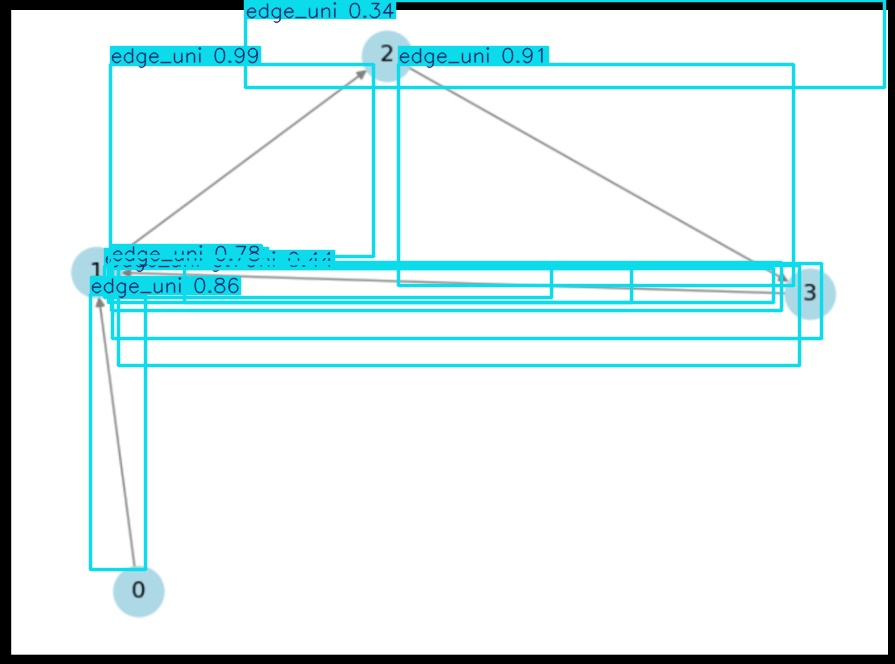
\includegraphics[width=0.5\textwidth]{test.jpg}
    \caption{YOLO edge detection: Even the bi-directional edges were treated as edge\_uni.}
    \label{fig:example}
\end{figure}

The next approach used was to detect lines and arrowheads separately. Annotations were done as "edge" for a line and "arrow" for an arrowhead. This model gave much better results, and due to the time constraint it was decided to be finalised.



The detailed models and their data may be accessed here:
\href{https://drive.google.com/drive/folders/1PqM-U-EIa0wvnxUx_WWJJRzeCGIo2qsN?usp=sharing}{YOLOv8s models}

For the training, 
\begin{itemize}
    \item 80 graphs were fed to the first model, and 100 to the second.
    \item The number of epochs was 100
    \item the batch size was taken 16.
    \item A yolov8s model was used.
\end{itemize}

This model would be called into the code and predictions would be done on the rest of the graphs. The problems that were discovered (and the strategy used to tackle each one of them) are listed in chronological order from this point.

\section{PART A1: Identifying Edges}

For this purpose, 
\begin{itemize}
    \item The yolov8 model was first called into the code.
    \begin{lstlisting}[language=Python, caption=Calling the model]
    from ultralytics import YOLO
    model_path = r"C:\Users\ADITYA\runs\detect\train4\weights\best.pt"
    \end{lstlisting}
    \item Then, the arrows and edges were extracted (with numbering, so that it would be easier to debug).
    \begin{lstlisting}[language=Python, caption=Gathering the arrows and edges. The graph was outputted in order to check for possible issues and their cause.]
    model = YOLO(model_path)
    results = model(image_path)[0]

    label_map = {0: "arrow", 1: "edge"}

    edges = []
    arrows = []
    h, w, _ = image.shape
    
    edge_counter = 1
    arrow_counter = 1
    
    for box in results.boxes.data.tolist():
        x1, y1, x2, y2, conf, cls = box[:6]
        cls = int(cls)
        x1, y1, x2, y2 = map(int, [x1, y1, x2, y2])
        label = label_map.get(cls, f"class_{cls}")
    
        if cls == 0:
            arrows.append((arrow_counter, [x1, y1, x2, y2]))
            label_text = f"arrow {arrow_counter}"
            arrow_counter += 1
            color = (0, 255, 0)
        elif cls == 1:
            edges.append((edge_counter, [x1, y1, x2, y2]))
            label_text = f"edge {edge_counter}"
            edge_counter += 1
            color = (0, 0, 255)
        else:
            label_text = f"{label} {conf:.2f}"
            color = (255, 0, 0)
    
        cv2.rectangle(image, (x1, y1), (x2, y2), color, 1)
        cv2.putText(image, label_text, (x1, y1 - 5), cv2.FONT_HERSHEY_SIMPLEX, 0.5, color, 1)
    \end{lstlisting}
    \item To calculate the direction of the arrows, the following idea was initially thought of:
    \begin{itemize}
        \item Firstly, we had to check along which diagonal the edge was (the bounding boxes were conveniently marked in the model such that the edges would be along diagonals).
        \item Then, we had to check the closest nodes along that edge
        \item Then, arrows were checked.
    \end{itemize}    
\end{itemize}

\section{PART A2: Optimization for edges}

Our pipeline for now is as follows:

The directionality of an edge is determined using a two-step process involving diagonal alignment and arrow proximity. First, for each YOLO-detected edge bounding box, two diagonals are considered: the primary diagonal from top-left to bottom-right $$(x_1, y_1)$$ to $$(x_2, y_2)$$ and the alternate diagonal from bottom-left to top-right $$(x_1, y_2)$$ to $$(x_2, y_1)$$. Each diagonal’s endpoints are compared to all detected node coordinates using the closest\_node\_to\_point() function, which calculates the Euclidean distance to identify the closest node to each endpoint. The total sum of distances for both diagonal endpoints to their respective closest nodes is computed for each diagonal, and the diagonal with the smaller total distance is selected as the likely connection, yielding a node pair (node\_a, node\_b). Then, to determine if this edge is directional, the midpoint of each YOLO-detected arrow bounding box is calculated and checked to see if it lies within the bounding rectangle of the edge. If so, the Euclidean distances from the arrow’s center to node\_a and node\_b are computed, and the node closer to the arrow is inferred to be the origin, with the arrow pointing toward the destination node. Accordingly, a directed edge is added to the graph using G.add\_edge(origin, destination). If no arrow overlaps the edge, it is treated as undirected.

\begin{lstlisting}[language=Python, caption=Edge finding]
for edge_idx, (x1, y1, x2, y2) in edges:
    diag1 = [(x1, y1), (x2, y2)]
    diag2 = [(x1, y2), (x2, y1)]

    n1_diag1 = closest_node_to_point(diag1[0], id_to_coords)
    n2_diag1 = closest_node_to_point(diag1[1], id_to_coords)
    dist_diag1 = np.linalg.norm(np.array(id_to_coords[n1_diag1]) - np.array(diag1[0])) + \
                 np.linalg.norm(np.array(id_to_coords[n2_diag1]) - np.array(diag1[1]))

    n1_diag2 = closest_node_to_point(diag2[0], id_to_coords)
    n2_diag2 = closest_node_to_point(diag2[1], id_to_coords)
    dist_diag2 = np.linalg.norm(np.array(id_to_coords[n1_diag2]) - np.array(diag2[0])) + \
                 np.linalg.norm(np.array(id_to_coords[n2_diag2]) - np.array(diag2[1]))

    if dist_diag1 <= dist_diag2:
        node_a, node_b = n1_diag1, n2_diag1
    else:
        node_a, node_b = n1_diag2, n2_diag2

    directed = False
    for arrow_idx, (ax1, ay1, ax2, ay2) in arrows:
        arrow_cx = (ax1 + ax2) // 2
        arrow_cy = (ay1 + ay2) // 2

        if min(x1, x2) <= arrow_cx <= max(x1, x2) and min(y1, y2) <= arrow_cy <= max(y1, y2):
            coord_a = id_to_coords[node_a]
            coord_b = id_to_coords[node_b]
            dist_to_a = np.linalg.norm(np.array([arrow_cx, arrow_cy]) - np.array(coord_a))
            dist_to_b = np.linalg.norm(np.array([arrow_cx, arrow_cy]) - np.array(coord_b))

            if dist_to_a < dist_to_b:
                G.add_edge(node_b, node_a)
            else:
                G.add_edge(node_a, node_b)

            directed = True
            break
\end{lstlisting}

However, it was quickly realised that with this, there was no limit as to how far a node would be detected. Sometimes, there were bounding boxes on partial edges that were giving trash data which caused more confusion. To avoid that, a threshold was introduced to first check whether there is a node in the range of that threshold, and if yes, then the closest\_node function was applied.

\section{PART A3: Treating bidirectionality}

To check for bidirectional arrows, it was necessary to ensure that arrows were checked on both sides of the endpoints of the bounding box. If an arrow was found on one of the sides, it would be considered unidirectional and if an arrow was found on both sides, it would be considered bidirectional.

However, a major problem came out during this step which could not be finally resolved: If an arrow from another edge was too close, it was getting included and unidirectional edges were also classified as bidirectional.

At this stage, the source code was tested on some of the graphs randomly and two main problems were gathered on debugging (by pringint out the edges detected and processing each edge):

\begin{itemize}
    \item Just like in Canny edge detection, some incomplete bounding boxes existed (covering partial edges) which was causing missing edges.
    \item  The problem mentioned above this.
\end{itemize}

\begin{lstlisting}[language=Python, caption=Debugs applied in the arrow logic to figure out issues]
    for arrow_idx, (ax1, ay1, ax2, ay2) in arrows:
        arrow_cx = (ax1 + ax2) // 2
        arrow_cy = (ay1 + ay2) // 2

        if min(x1, x2) <= arrow_cx <= max(x1, x2) and min(y1, y2) <= arrow_cy <= max(y1, y2):
            print(f"  Overlapping arrow {arrow_idx} | Center: ({arrow_cx},{arrow_cy})")

            dist_to_a = np.linalg.norm(np.array([arrow_cx, arrow_cy]) - np.array(corner_a))
            dist_to_b = np.linalg.norm(np.array([arrow_cx, arrow_cy]) - np.array(corner_b))

            if dist_to_a <= ARROW_MATCH_THRESHOLD:
                print(f"   Arrow {arrow_idx} is near node {node_a} (distance={dist_to_a:.1f} <= {ARROW_MATCH_THRESHOLD})")
                arrows_near_a.append(arrow_idx)
            else:
                print(f"    Arrow {arrow_idx} rejected for node {node_a} (distance={dist_to_a:.1f} > {ARROW_MATCH_THRESHOLD})")

            if dist_to_b <= ARROW_MATCH_THRESHOLD:
                print(f"    Arrow {arrow_idx} is near node {node_b} (distance={dist_to_b:.1f} <= {ARROW_MATCH_THRESHOLD})")
                arrows_near_b.append(arrow_idx)
            else:
                print(f"    Arrow {arrow_idx} rejected for node {node_b} (distance={dist_to_b:.1f} > {ARROW_MATCH_THRESHOLD})")

    if arrows_near_a and not arrows_near_b:
        print(f"  Direction inferred: {node_b} -> {node_a} (arrow(s) near node {node_a} only)")
        G.add_edge(node_b, node_a)
    elif arrows_near_b and not arrows_near_a:
        print(f"  Direction inferred: {node_a} -> {node_b} (arrow(s) near node {node_b} only)")
        G.add_edge(node_a, node_b)
    elif arrows_near_a and arrows_near_b:
        print(f"  Bidirectional edges inferred (arrows near both nodes)")
        G.add_edge(node_a, node_b)
        G.add_edge(node_b, node_a)
    else:   
        print("  No arrows near endpoints - treating as undirected (both ways)")
\end{lstlisting}

\section{PART A4.1: Optimizations tried for Incomplete boxes}

The model "Strat 2" (part of the YOLO drive link above) was initially trained on 50 images. It was observed that the edges that were getting chunked/missed out were larger edges. One method to approach this was to expand the dataset and see if the accuracy improves. However, there was no improvement seen when 100 images were sent in instead of 50. 

\begin{figure}[h!]
    \centering
    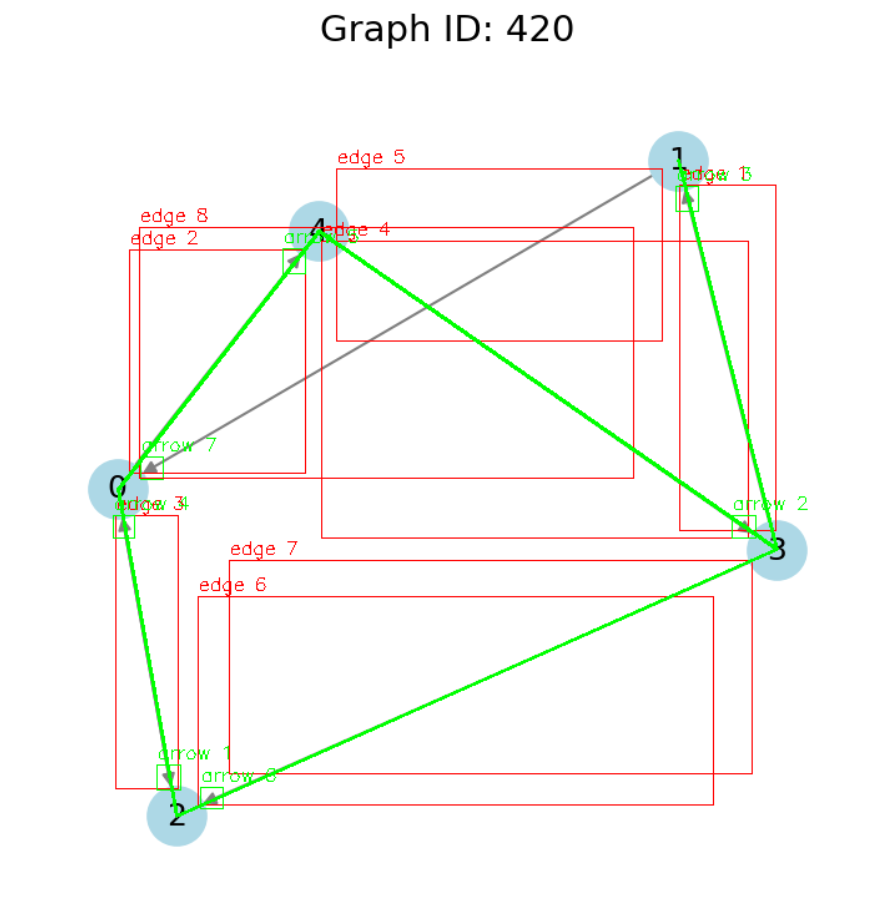
\includegraphics[width=0.5\textwidth]{420.png}
    \caption{Partial boxes causing an edge to be missed out.}
    \label{fig:example}
\end{figure}

The next optimization applied was to essentially remove noise by merging partial edges into a full edge. For this- various parameters had to be checked:

\begin{itemize}
    \item Is the slope of the line similar? Can the two be considered parallel? The slope was calculated by the equation $$m = (y_2 - y_1)/(x_2 - x_1)$$, where the endpoints of the bounding box were fed in as coordinates.
    \item Is the line close enough to actually align? What is the perpendicular distance between the extended lines?
    \item What must be the threshold to consider bounding boxes to be merged? How would it be ensured that extra boxes are not merged unnecessarily?
\end{itemize}

After some research, it was decided to use the ratio of the overlap area and the combined area of the two rectangles as a parameter, also known as the IOU (Intersection Over Union). $$IOU = Area(overlap)/Area(combined)$$.

\begin{lstlisting}[language=Python, caption=Algorithm to merge and complete edges]
def compute_iou(boxA, boxB):
    xA = max(boxA[0], boxB[0])
    yA = max(boxA[1], boxB[1])
    xB = min(boxA[2], boxB[2])
    yB = min(boxA[3], boxB[3])
    interArea = max(0, xB - xA) * max(0, yB - yA)
    boxAArea = (boxA[2] - boxA[0]) * (boxA[3] - boxA[1])
    boxBArea = (boxB[2] - boxB[0]) * (boxB[3] - boxB[1])
    return interArea / float(boxAArea + boxBArea - interArea + 1e-6)

def merge_boxes(boxes):
    x1 = min(box[0] for box in boxes)
    y1 = min(box[1] for box in boxes)
    x2 = max(box[2] for box in boxes)
    y2 = max(box[3] for box in boxes)
    return [x1, y1, x2, y2]

merged_edges = []
used = [False] * len(edges)
for i in range(len(edges)):
    if used[i]:
        continue
    group = [edges[i][1]]
    merged_ids = [edges[i][0]]
    used[i] = True
    for j in range(i+1, len(edges)):
        if used[j]:
            continue
        if compute_iou(edges[i][1], edges[j][1]) > MERGE_IOU_THRESHOLD:
            group.append(edges[j][1])
            merged_ids.append(edges[j][0])
            used[j] = True
    merged_bbox = merge_boxes(group)
    merged_edges.append((len(merged_edges) + 1, merged_bbox))
\end{lstlisting}

\begin{figure}[h!]
    \centering
    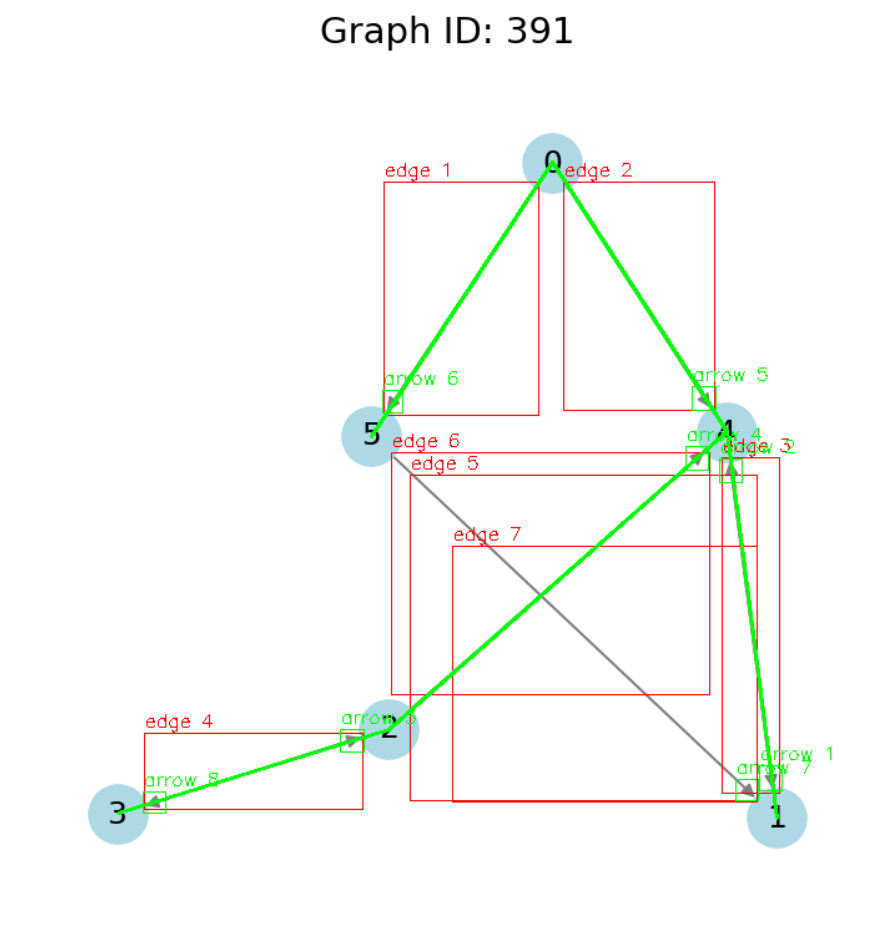
\includegraphics[width=0.5\textwidth]{391_before.png}
    \label{fig:example}
\end{figure}

\begin{figure}[h!]
    \centering
    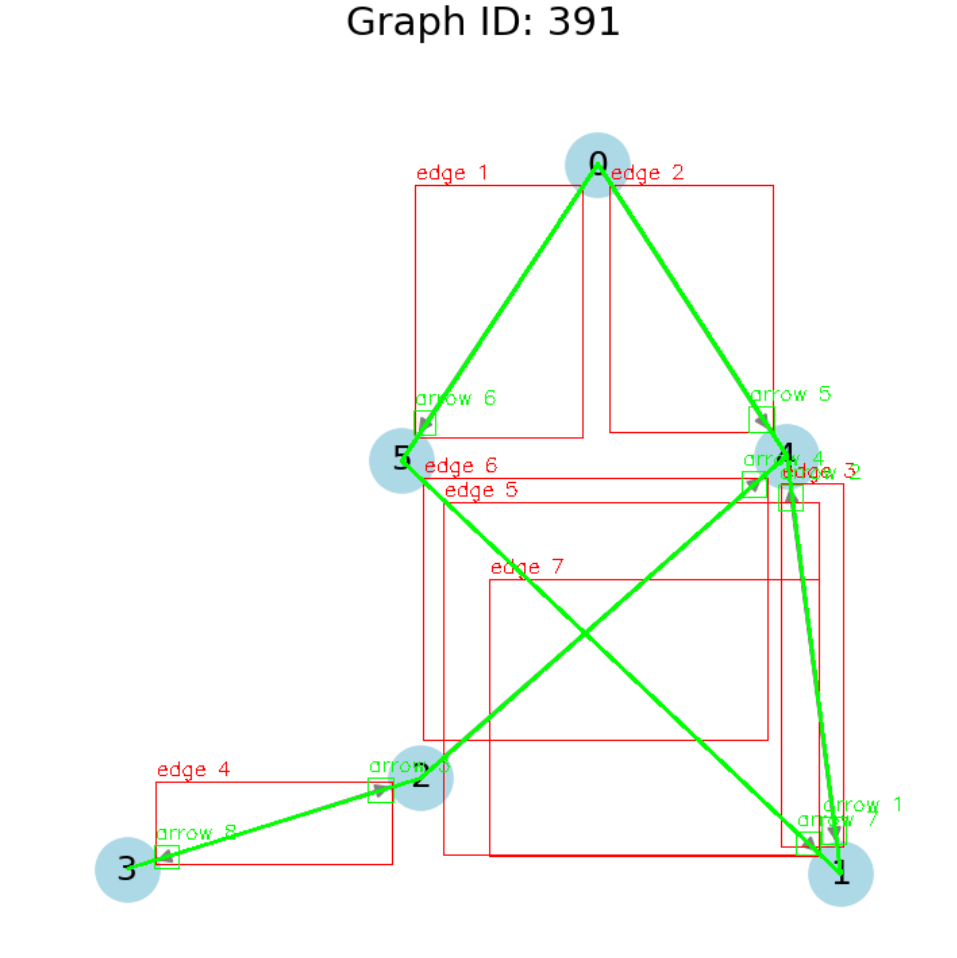
\includegraphics[width=0.5\textwidth]{391_after.png}
    \caption{Analysis of Graph 391 after applying the preprocessing steps, but before and after the IOU condition was applied and integrated. Similar results were seen for a few more graphs as well.}
    \label{fig:example}
\end{figure}

The operation would be as follows:
\begin{itemize}
    \item Process the graph once before merging edges
    \item Merge the edges and process it again
    \item Take the union of both of the processed outputs so that no edges are excluded
\end{itemize}

This step improved the accuracy significantly, but not always.

\section{PART A4.2: Possible optimization for accuracy of arrow detection}

This optimization was not implemented successfully due to time constraints.

\begin{itemize}
    \item We detect the edges before and after merging as earlier, but with a small change: Only the raw edges with the endpoints are detected, without the direction processing.
    \item Before the direction processing, we can extract each bounding box from the final union of raw edges, and apply Canny Edge detection or skeletonization on that small extracted box.
    \item Since the section within the bounding box is much smaller and less comples, it is expected that such methods will be able to show good accuracy. 
\end{itemize}

\section{PART B: Finding Shortest Path} 

This is a much less sophisticated part, and was seen as a shortest path CP problem with the additional "jamming" constraint of node reversal. We use the following strategy:

\begin{itemize}
    \item The edges are known and can be taken from an input file.
    \item We construct the graph using an adjacency matrix. Note that we also need to store the graph with reversed edges as another adjacency matrix in this case.
    \item Then, we need to find the shortest path. To handle the additional constraint of jamming, we would need to use a combination of Dijkstra's Algorithm and dynamic programming as follows:
    \begin{itemize}
        \item Let dp[i][j] be the fuel required to reach node i when you are currently in state j. Here, j = 0 when the graph is as it is and j = 1 when the graph is reversed.
        \item Initially, all the fuel values are set to LLONG\_MAX.
        \item As the algorithm progresses, it performs a variant of Dijkstra’s shortest path search over this graph.
        \item Whenever a path with a smaller fuel cost to a particular node and state is found, the dp value is updated, and the corresponding node-state pair is pushed into the priority queue for further exploration.
        \item If no path is found, the output would be -1.
    \end{itemize}
\end{itemize}

\begin{lstlisting}[language=C++, caption=Algorithm to calculate fuel cost]
int main() {
    fastio;

    ifstream fin("graph.txt");
    vector<pi> edges;
    int a, b;
    int max_node = 0;
    while (fin >> a) {
        if (a == -1) break;
        fin >> b;
        edges.emplace_back(a, b);
        max_node = max({max_node, a, b});
    }
    int n = max_node + 1;

    vector<vi> adj[2];
    adj[0].resize(n);
    adj[1].resize(n);
    for (auto [u, v] : edges) {
        adj[0][u].push_back(v);
        adj[1][v].push_back(u);
    }

    using State = tuple<ll, int, int>;
    priority_queue<State, vector<State>, greater<State>> pq;
    vector<vector<ll>> dp(n, vector<ll>(2, LLONG_MAX));
    dp[0][0] = 0;
    pq.emplace(0, 0, 0);

    while (!pq.empty()) {
        auto [cost, u, s] = pq.top();
        pq.pop();

        if (u == n - 1) {
            cout << cost << endl;
            return 0;
        }

        if (cost > dp[u][s]) continue;

        for (int v : adj[s][u]) {
            ll new_cost = cost + 1;
            if (new_cost < dp[v][s]) {
                dp[v][s] = new_cost;
                pq.emplace(new_cost, v, s);
            }
        }

        int new_s = 1 - s;
        ll new_cost = cost + n;
        if (new_cost < dp[u][new_s]) {
            dp[u][new_s] = new_cost;
            pq.emplace(new_cost, u, new_s);
        }
    }

    ll ans = min(dp[n-1][0], dp[n-1][1]);
    if (ans == LLONG_MAX) {
        cout << -1 << endl;
    } else {
        cout << ans << endl;
    }
\end{lstlisting}

Examples:
\begin{lstlisting}[caption=Example Input 1]
0 1
1 2
2 3
3 1
\end{lstlisting}
\begin{lstlisting}[caption=Example Output 1]
3
\end{lstlisting}
In this case, the graph can be traversed as 0--1--2--3, taking 3 fuels.
\begin{lstlisting}[caption=Example Input 2]
0 1
2 1
2 3
4 3
3 5
\end{lstlisting}
\begin{lstlisting}[caption=Example Output 2]
29
\end{lstlisting}
In this case, the graph can be traversed as 0--1-(reverse)-2-(reverse)-3-(reverse)-4-(reverse)-5, making the total cost 6*4 + 5 = 29.

\section{PART C: Discussing how to use and further notes}
The user would have to input their graph into image\_path, followed by which a txt file "graph.txt" is outputted on running the python source code. Then, the C++ source code for calculating shortest distance must be opened in the same directory and run. The C++ code takes graph.txt as input and returns the output in the terminal.

\textbf{The accuracy of detecting individual directed edges is expected to be  around 90\% using this pipeline, and 97-98\% if the edge lengths are small.}

Some further optimizations include:
\begin{itemize}
    \item Using a CNN model and training it specifically for node and edge detection to improve accuracy and robustness over classical methods like HoughCircles or heuristic thresholds.
    \item  Optimizing the bounding box merging logic by integrating IOU thresholds dynamically based on detection confidence or spatial distribution.
\end{itemize}

An alternative pipeline that was also thought of is shortly explained below:
\begin{itemize}
    \item Do the detections as done earlier, but with a constraint: Consider only the edges having an inclination magnitude between a certain threshold angle (e.g: 20 to 70 degrees)
    \item This is because it was observed that errors in arrow detection and inaccuracies in bounding boxes were high when the edges were close to being horizontal or vertical.
    \item Then, rotate the image by 45 degrees and apply the same process over again.
    \item Combine the results obtained from both of these.
\end{itemize}

The optimizations and the other pipeline can potentially be tested in the future.








\end{document}
